\documentclass[a4paper,czech]{article}
\usepackage[T1]{fontenc}
\usepackage[utf8]{inputenc}
\usepackage[czech]{babel}

\usepackage{anysize}
\usepackage{geometry}
%\geometry{a4paper, portrait, margin=2.5cm}

\usepackage{graphicx} % Required for the inclusion of images
\usepackage{amsmath} % Required for some math elements 
\usepackage{fancyhdr} %na headers
\usepackage{multirow}
\usepackage{caption}
\usepackage[colorlinks=false,unicode=true]{hyperref}
\usepackage{indentfirst}
\usepackage{tikz}
\graphicspath{ {images/} }

%\setlist[enumerate]{label*=\arabic*.}
%\setlength\parindent{0pt} % Removes all indentation from paragraphs

\renewcommand\familydefault{\sfdefault}
%\renewcommand{\sectionmark}[1]{\uppercase{\markboth{}{\emph{~#1}}}}
%\renewcommand{\subsectionmark}[1]{}% Remove \subsection from header
\def\tableautorefname{tab.}
\def\figureautorefname{obr.}
\def\sectionautorefname{kap.}
\def\equationautorefname{rovn.}
\def\subsectionautorefname{podkap.}

\begin{document}

\LARGE{\textbf{Otázky na TBK 2018}}
\newpage
\section{Úvod}
\subsection{\textbf{Vyjmenujte alespoň 5 příkladů běžně používaných bezdrátových komunikačních systémů. Najděte k nim pracovní frekvenční pásma.}}

\section{Systémy}
\subsection{\textbf{Nakreslete blokové schéma RX s 2-násobným směšováním a popište funkci.}}
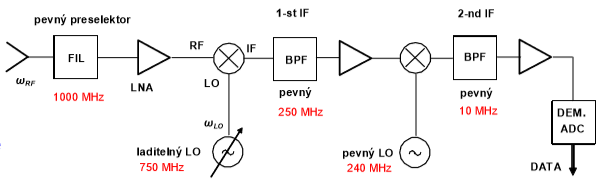
\includegraphics{images/rx_2_nasobny.png}
\begin{itemize}
	\item Používá se vysoká frekvence 1. IF filtru $\omega_IF1$
	\item Zrcadlové pásmo je potom vzdálené a dá se dobře filtrovat, lze použít jednoduchý filtr na fixní frekvenci
	\item Další zpracování na vysoké frekvenci $\omega_IF1$ je neefektivní (horší parametry demodulátoru, vyšší nároky a ADC, ...) a proto se používá 2. přídavný směšovací stupeň.
\end{itemize}
\subsection{\textbf{Nakreslete blokové schéma přijímače s přímou konverzí do základního pásma. Jaké jsou výhody a nevýhody této struktury.}}
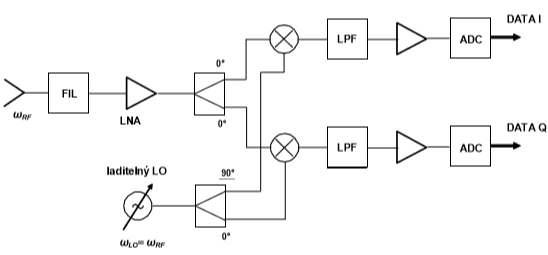
\includegraphics{images/tx_priama_konv.png}
\begin{itemize}
	\item\textit{Výhody}
		\subitem Širokopásmový príjem -> malá HW omezení
		\subitem Relativně jednoduché, malé rozměry, nízký DC příkon, cena, ...
		\subitem ADC pracují na nízkých frekv. -> výhodné parametry, cena
		\subitem Demodulace je prováděna v digitální doméně -> odpovídá koncepci (SDR – software defined radio), lze jednoduše modifikovat
		\subitem Lze měnit $$B_M=B_IF$$
\end{itemize}
\subsection{\textbf{Co to je transceiver? Jaký je rozdíl mezi duplexerem a diplexerem? Jak je možné konstruovat diplexery?}}
\begin{itemize}
	\item \textbf{Duplexer} - zařízení používané v systémech používajících full nebo half duplex kdy je nutno sloučit TX a RX do jedné antény -> slučovač
	\item \textbf{Diplexer} - zařízení zestávajíci z dvou filtrů, umožnující dvoum signálům o dostatečně vzdálených frekvencích sdílet jeden komunikační kanál (anténu), je možné jej konstruovat kombinací dolní propusti a horní propusti nebo 2 pásmových propustí s rozdílnými propustnými pásmy na $\omega_{TX}$ a $\omega_{RX}$
\end{itemize}
\subsection{\textbf{Vysvětlete techniky TDD a FDD.}}
\begin{itemize}
	\item \textbf{TDD} - technologie duplexerů, která používá vysokofrekvenční přepínače (FET, PIN), je to jednoduché a efektivní řešení, ale s nízkou přenosovou rychlostí.
	\item \textbf{FDD} - technologie duplexerů, která používá diplexery-slučovací filtry, RX a TX mohou pracovat 100\% času tedy dosahujeme plný duplex při splnění požadavků diplexeru.
\end{itemize}

\section{Měření}
\subsection{\textbf{Popište sestavu skalárního analyzátoru.}}
\begin{itemize}
	\item vyhodnocovací jednotka -> DC zesilovač, ADC, display, DSP, klávesnice,...
	\item generátor
	\item 1-2 detektor
	\item směrový můstek nebo směřová vazba
	\item propojovací kabely, adaptéry, attenuátory.
\end{itemize}
\subsection{\textbf{Jak se provádí kalibrace a měření přenosu a odrazů pomocí skalárního analyzátoru? }}
\begin{itemize}
	\item kalibrace se provádí tak, že detektor měří na všech frekvencích $P_{in}$ a hodnoty ukládá do paměti, je potřeba kalibr $L=0$ kdy platí $P_{out}=p_{in}$ v praxi se používá krátký úsek TL nebo propojka.
	\item při měření zisku detektor měří $P_{out}$
	\item $G=\frac{P_{out}}{P_{in}}$ - zisk
	\item \textbf{RL} - return loss -> o kolik dB je výkon vlny odražené nižší, než je výkon vlny dopadající $RL = -10\log(\frac{P_b}{P_a}=-(P_{bdBm}-P_{adBm})$
	\item pro měření odražené vlny b lze použít:
	\subitem směrovou vazbu
	\subitem směrový můstek
\end{itemize}
\subsection{\textbf{Jak fungují senzory používané pro měření přenosu a odrazů pomocí skalárního analyzátoru? }}
\begin{itemize}
	\item \textbf{Wheastoneov můstek} - je modifikovaný, na diagonále má $50 \Omega$
	\subitem rozdílové napětí se měří ZBS detektorem, výstupní DC napětí je odděleno odpory s hodnotami řádově $k\Omega$
	\subitem pokud je identická bezodrazová koncovka na bráně TEST tak je můstek vyvážený, $V_{diff}=0$
	\subitem ak je $Z_{DUT}\neq Z_0 \to V_{dif}\neq 0$
	\item \textbf{Směrová vazba} - 3 bran schopný oddělit dopadající a odraženou vlnu
	\subitem vlna $a_G$ projde DCp a na bráně 1=TEST vytváří dopadající vlnu $a$
	\subitem výkon navázané části vlny $b \to b_c$ je měřen DET
\end{itemize}
\subsection{\textbf{Popište základní principy funkce vektorových analyzátorů obvodů VNA}}
\begin{itemize}
	\item měří s-parametry - koeficienty přenosu a odrazu včetně fází, má velmi efektivní korekci vlivu všech komponent v měřící trase
	\item \textbf{měření $s_{11} \text{ a } s_{21}$}
	\begin{itemize}
		\item jednotka 8753C má 1 výstup (S="source"=generátor) a 3 vstupy (přijímače typu superhet)
		\item signál z výstupu S je rozdělen do větve R a do větve PORT1
		\item přijímač R měří dopadající vlnu $a_1$
		\item směrová vazba DCp1 navazuje -6 dB vzorek vlny $b_1$ na vstup přijímače A
		\item směrová vazba DCp2 navazuje -6 dB vzorek vlny $b_2$ na vstup přijímače B
		\item DSP vyhodnocuje $s_{11} \text{ a } s_{21}$
	\end{itemize}
	\item \textbf{měření $s_{22} \text{ a } s_{12}$}
	\begin{itemize}
		\item přijímač R měří dopadající vlnu $a_2$
		\item směrová vazba DCp1 navazuje -6 dB vzorek vlny $b_1$ na vstup přijímače A
		\item směrová vazba DCp2 navazuje -6 dB vzorek vlny $b_2$ na vstup přijímače B
		\item DSP vyhodnocuje $s_{22} \text{ a } s_{12}$
	\end{itemize}
\end{itemize}
\subsection{\textbf{Proč a jak se provádí kalibrace a korekce VNA pro měření odrazů?}}
\begin{itemize}
	\item provádí se pro odstranění vlivu komponent měřící sestavy pomocí SW
	\item můžeme použít mnoho různých metod - TRL, SOLT,...
	\item Příklad kalibrace VNA - měření 1-branu
	\begin{itemize}
		\item vyžaduje 3 komplexní kalibry (nejčastěji OPEN, SHORT, MATCH)
		\item z měření kalibrů lze určit s-parametry chybového 2-branu a výpočtem provést úplnou koreci
	\end{itemize}
\end{itemize}
\subsection{\textbf{Nakreslete a popište základní blokové schéma spektrálního analyzátoru SpA}}
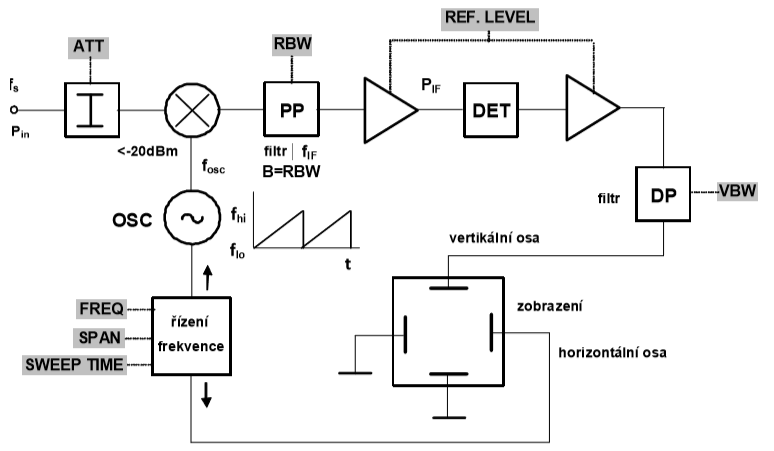
\includegraphics[width=\textwidth,keepaspectratio]{images/SpA.png}
\begin{itemize}
	\item vstupní attenuátor zabezpečuje dostatečne nízký výkon na vstupu (typ. -20dBm) 1. směšovače $\to$ nízké vnitřní IM produkty SpA
	\item Směšovač konvertuje vstupní signál s frekvencí $f_s$ (přeladění je široké \textbf{SPAN}) do pevného IF filtru na frekvenci $f_{IF}$, šířka IF filtru je B=\textbf{RBW} - definuje měřící okno SpA
	\item přeladění řídí osciloskop který generuje signál s frekvencí $f_{OSC}$použitá frekvenční konverze je pak $f_{IF} = f_s-f_{OSC}$
	\item OSC se přelaďuje do $f_{LO}$ do $f_{hi}$, řízeno nastavením \textbf{FREQ} a \textbf{SPAN}
\end{itemize}
\subsection{\textbf{Princip měření spektra pomocí SpA}}
\begin{itemize}
	\item SpA přejíždí frekvenční pásmo \textbf{SPAN} měřícím oknem širokým \textbf{RBW}. V každém frekvenčním bodu zobrazení(celkem typ. N=400 bodů) přístroj měří výkon v okně širokém RBW a zobrazí hodnotu na displeji.
	\item Měřené frekvenční pásmo je určeno nastavením \textbf{FREQ-CENTER}(frekv. odpovídající středu zobrazení) a SPAN 
\end{itemize}
\subsection{\textbf{Co to je šumový práh SpA? Jak optimálně nastavíte SpA pro měření velmi slabých signálů?}}
\begin{itemize}
	\item je to citlivost
	\item pro měření velmi slabých signálů nastavíme \textbf{ATT} na 0
\end{itemize}
\subsection{\textbf{Jaký rozdíl je mezi RBW a VBW a jaký mají tato nastavení vliv na měření pomocí SpA?}}
\begin{itemize}
	\item \textbf{RBW} - šířka frekvenčního okna, filtr s nějakou šířkou pásma
	\item \textbf{VBW} - šířka DP filtru za detektorem, snižuje šp-šp amplitudu a nemění šumový práh
\end{itemize}
\subsection{\textbf{Vysvětlete nastavení FREQ-CENTER, SPAN, REFERENCE LEVEL, SWEEP TIME, ATT. Jaký vliv mají na měření pomocí SpA?}}
\begin{itemize}
	\item \textbf{REFERENCE LEVEL} - vstupní VF výkon odpovídající horní vodorovné ose
	\item \textbf{SWEEP TIME} - doba 1 zobrazení, závisí na RBW a SPAN
	\item ostatné viz. predchádzajúci text
\end{itemize}

\section{Antény}
\subsection{\textbf{Co vyjadřuje teorém reciprocity antény?}}
\begin{itemize}
	\item 
\end{itemize}
\subsection{\textbf{Jak je definována vstupní impedance antény?}}
\begin{itemize}
	\item je to impedance, kterou by jsme naměřili na vstupních svorkách antény
	\item sestává z odporu záření $R_{vyz}$, ze ztrátového odporu $R_{ztr}$ a z reaktance záření $X_A$
	\item $Z_A = (R_{vyz} + R_{ztr}) + iX_A$
\end{itemize}
\subsection{\textbf{Co je to vyzařovací odpor antény?}}
\begin{itemize}
	\item je hodnotou reálného odporu v kmitně proudu antény. Je tedy jednou ze složek (té reálné) vstupní impedance v kmitně proudu.
\end{itemize}
\subsection{\textbf{Jak lze pomocí náhradního obvodového schématu antény vyjádřit vyzářený výkon?}}
\begin{center}
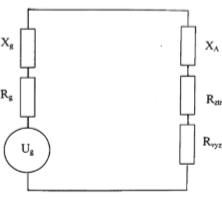
\includegraphics{images/ant_nahr.png}
\end{center}
\begin{itemize}
	\item $P_{vyz} = \frac{1}{2}|I_g|^2R_{vyz}=\frac{|U_g|^2}{2}[\frac{R_{vyz}}{(R_{vyz}+R_{ztr}+R_g)^2+(X_A+X_g)^2}]$
\end{itemize}
\subsection{\textbf{Jak lze pomocí náhradního obvodového schématu antény vyjádřit výkon ztracený na anténě přeměnou na teplo?}}
\begin{itemize}
	\item $P_{ztr} = \frac{|U_g|^2}{8}[\frac{R_{ztr}}{(R_{vyz}+R_{ztr})^2}]$
\end{itemize}
\end{document}
